\chapter{Focal Length}

\section{Aim}
To learn how determine the focal length of a convex lens

\section{Background Information}
Lenses are transparent curved objects which tend to bend light. A convex lens is one which bends the light towards a common point, called the focal point. The focal length is the distance from the middle of the lens to the focal point. The focal length of an optical instrument is a measure of how strongly the lenses converges or diverges light. Lenses are commonly used in cameras, spectacles, telescopes, binoculars and many other optical instruments. Therefore, it is important to determine the focal length of a lens to know how to construct an optical instrument best.

\section{Materials}
Optical bench, source of light, optical pin, pin holder, screen, convex lens, lens holder

\section{Procedure}
\begin{enumerate}
\item Fix the source of light on an optical bench.
\item Fix an optical pin upright in pin holder and place it close to the front side of the source of light.
\item Place a screen a distance from the pin.
\item Fix the convex lens on a lens holder.
\item Place the lens holder between the optical pin and the screen.
\item Adjust the lens holder along the optical bench until a sharp image is obtained on the screen (see figure).
\item Measure the distance from the optical pin to the lens holder and record it as $u$.
\item Measure the distance from the lens holder to the screen and record it as $v$.
\item Change the position of optical pin to obtain five (5) more values of $u$ and $v$, tabulate the results.
\end{enumerate}

\begin{figure}[h!]
\centering
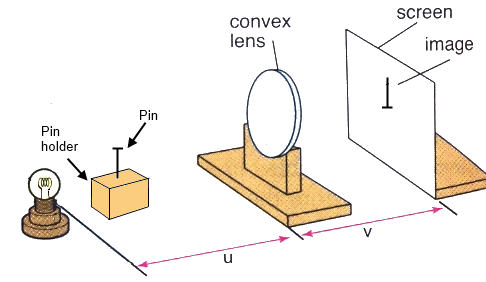
\includegraphics[width=10cm]{./img/focal-length-1.png}
\caption{Focal Length practical setup}
\label{fig:focal-length-1}
\end{figure}

\section{Analysis and Interpretation}
\begin{enumerate}
\item From the table compute values of $^1/_v$ and $^1/_u$.
\item Plot a graph of $^1/_v$ against $^1/_u$.
\item What is the value of the vertical-intercept of the graph?
\item Find the slope of the graph.
\item If the vertical intercept is equal to $^1/_f$, where $f$ is the focal length, deduce the equation of the graph.
\end{enumerate}

\section{Conclusion}
What is the focal length of the lens used?

\section{Questions for Discussion}
\begin{enumerate}
\item Farsighted individuals have an eye focal length which is too long. What type of lens could be used in front of their eyes to help them focus the light properly?
\item What is the relationship between the power of the lens and focal length?
\end{enumerate}

\section{Reflection and Self Assessment}
\begin{enumerate}
\item Explain other methods which can be used to determine the focal length of a lens?
\item Do you understand the results of this experiment? If not, in what ways can you improve your understanding?
\end{enumerate}